%
%
\section{Grundlegender Aufbau und Ziel der Beispielanwendung}
%
%
\subsection{Allgemeines}
Um die Funktionsweise des MyCoRe-Kernes zu testen wurde eine Beispielanwendung basiered auf diesem Kern entwickelt. Sie soll dem Anwender eine voll funktionsf"ahige Applikation in die Hand geben, welche eine Vielzahl von Komponenten des MyCoRe-Projektes nutzt und deren Arbeitweise klar werden l"asst. Um die Anwendung, im weiteren MyCore-Sample genannt, gleichzeitig sinnvoll einsetzten zu k"onnen, wurde als Beispielszenario ein Dokumentserver gew"ahlt, wie er bei vielen potentiellen Nutzern zur Anwendung kommt. Auch soll das MyCore-Sample die Nachfolge des erfolgreichen MILESS-Dokumentservers sein und den Migrationspfad zu MyCoRe hin aufzeigen. \\[2ex]
Analog zum MILESS werden auch hier die Metadaten in drei Gruppen aufgeteilt und von den eigentlichen multimedialen Objekten getrennt behandelt. Zur Modellierung des Datenmodells f"ur die Multimedia-metadaten wurde das allgemein verbreitete Dublin Core Datenmodell herangezogen und umgesetzt. Zur Realisierung wurden folgende Metadaten-Objekte entwickelt:
\begin{itemize}
\item {\bf Document} - Dieses Objekt beinhaltet die eigentlichen Metadaten des Multimedi-Objektes, in unserem Fall im Dublin Core Format, sowie Verweise auf extern gehaltene Daten wie die drei im weiteren genannten. Das Datenmodell besteht aus 15 Feldern, zur Speicherung verschiedener Datentypen gibt es atomare Grundkomponenetn. Weiterhin beinhalten die Metaddaten noch Teile zu ihrer Struktur und Verwaltung.
\item {\bf Klassifikation} - Hier k"onnen lineare oder hierarchich strukturierte Klassifikationen mit ihren Kategorien abgelegt werden. Jeder Verweis auf eine solche Kategorie aus einem Dokument heraus erfolgt mittels der ID der selben und nat"urlich der ID der Klassifikation als Identifiziererpaar. F"ur die Gestaltung der Klassifikationen wurde ein eigens Datenmmodel entwicklet.
\item {\bf LegalEntity} - Auch diese Metadaten sind analog dem {\bf Document} aus atomaren Komponenten zusammengesetzt und repr"asentieren nat"urliche und juristische personen, wie Autoren oder Einrichtunge.
\item {\bf Derivate} - Hinter diesem Begriff verbergen sich Darstellungsformen der eigentlichen multimedialen Objekte. Beispielsweise k"onnen das verschieden Dateiformate eines Images sein. Diese werden an das eigentliche Dokument gebunden.
\end{itemize}
Eine "Ubersicht zu den Beziehungen der Objektteile zueinander soll die folgende Grafik vermitteln. Wir haben uns aus den guten Erfahrungen von MILESS herraus entschlossen, diese Aufteilung beizubehalten, da so Einzelkomponeneten in Projekten schon geladen werden k"onnen, bevor andere Teile, z. B. das Scannen, abgeschlossen sind. \\
\begin{figure}[H]
\begin{center}
\fbox{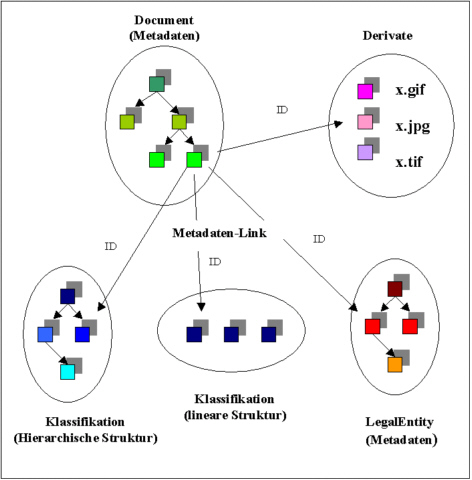
\includegraphics[scale=0.8]{UserGuide_3Goals_Pic01.jpg}}
\caption{"Ubersicht der Objekte im MyCoRe-Sample}
\end{center}
\end{figure}
Wie man der Grafik entnehmen kann, ist es m"oglich, neben Kategorien in Klassifikationen auch Metadaten der Documnets und LegalEntities hierarchich ineienander zu verschachteln. Auf dieser Basis k"onnen dann Strukturen wie z. B. die eines Buches abgebildet werden. Alle Beziehungen zwischen den Metadaten sind "uber eine eindeutige MCRObjectID gel"ost. \\
\subsection{Die MCRObjectID}
Dreh- und Angelpunkt aller Beziehungen von Metadaten und der daran angekn�pften Objekte ist ein eindeutiger Identifizierer. Im Falle des MyCoRe Projektes hat dieser den Namen {\bf MCRObjectID} erhalten. Er hat f�r alle Matadaten einen einheitlichen Aufbau und wird st�ndig zur Identifizierung genutzt. Auch das API des Systems bietet die M�glichkeit, diese ID automatisch zu generieren.\footnote{Siehe Programmers Guide.} Der Syntax der {\bf MCRObjectID} ist wie folgend festgelegt:\\
\begin{center}
{\bf MCRObjectID = {\it project\_type\_number}}
\end{center}
{\it project} - Dieses Element der ID spezifiziert ein bestimmtes Projekt. Es dient dazu, Daten verschiedener Projekte, welche sich gemeinsam auf einem System befinden, zu unterscheiden. Der Projektname sollte eindeutig sein und besteht aus einem Wort {\bf ohne Sonderzeichen}. Achten Sie immer darauf, dass Sie sich bei Vorhaben mit mehreren MyCoRe-Partnern von Anfang an auf einen Namen pro Projektteilnehmer verst�ndigen. F�r unser Sample haben wir {\bf MyCoReDemoDC} ausgew�hlt. {\bf Dieser Teil der ID ist case sensitive!}\\[2ex]
{\it type} - Jedem Metadatentyp des Datenmodells ist ein Typbezeichner zuzuordnen. Dieser stellt in MyCoRe die Verbindung von der Konfiguration des Metadatums bis hin zu dessen Suche und Pr�sentation dar. Der Typname der MCRObjectID wird immer in Kleinbuchstaben (lower case) innerhalb des Systems verwendet. Achten Sie von Anfang an darauf, dies umzusetzen. Im MyCoRe-Projekt gibt es reservierte Typnamen, diese sind\\
\begin{itemize}
\item {\bf class} - f�r Klassifikationen
\item {\bf derivate} - f�r Derivate
\end{itemize}
Zur Umsetztung des Datenmodells wurden weiterhin die Typen {\bf document} f�r Dokumente und {\bf legalentity} f�r Personen verwendet.
{\it number} - Dieser Teil dient der Identifizierung des Einzelobjektes. Es d�rfen nur nat�rliche Zahlen angegeben werden. Planen Sie Ihre Vergabe der Nummern bei eigenen Objekten sorgf�ltig. Da die Nummern teilweise als Strings verarbeitet werden, ist es sinnvoll, sie mit einer ausreichenden Zahl von Vornullen zu versehen. Dies erledigt das MyCoRe-System automatisch unter Zuhilfenahme des Konfogurationswertes {\tt MCR.metadata\_objectid\_number\_pattern } im File {\it mycore.properties.private }.
\subsection{Das Sample-Datenmodell}
Das Datenmodell des MyCoRe-Samples soll exemplarisch einen kleinen Dokumentserver abbliden, wie er dann f�r gro�e L�sungen �bernommen werden kann. Dabei sollen Multimediale Objekte verschiedenster Art und Herkunft gemeinsam verwaltet werden.
